\documentclass{article}%
\usepackage[T1]{fontenc}%
\usepackage[utf8]{inputenc}%
\usepackage{lmodern}%
\usepackage{textcomp}%
\usepackage{lastpage}%
\usepackage[head=40pt,margin=0.5in,bottom=0.6in]{geometry}%
\usepackage{graphicx}%
%
\title{\textbf{Gobierno desmejoró las escalas salariales del sector público desde 2007}}%
\author{ANA DÍAZ | anadiaz@el{-}nacional.com}%
\date{19/09/2018}%
%
\begin{document}%
\normalsize%
\maketitle%
\textbf{URL: }%
http://www.el{-}nacional.com/noticias/economia/gobierno{-}desmejoro{-}las{-}escalas{-}salariales{-}del{-}sector{-}publico{-}desde{-}2007\_252283\newline%
%
\textbf{Periodico: }%
EN, %
ID: %
252283, %
Seccion: %
Economía\newline%
%
\textbf{Palabras Claves: }%
NO\_TIENE\newline%
%
\textbf{Derecho: }%
2.3%
, Otros Derechos: %
NO\_TIENE%
, Sub Derechos: %
2.3.4%
\newline%
%
\textbf{EP: }%
NO\newline%
\newline%
%
\textbf{\textit{El instructivo, no publicado aún en Gaceta Oficial, rebajó o eliminó primas y compensaciones que elevaban el ingreso global de los trabajadores, denunciaron dirigentes}}%
\newline%
\newline%
%
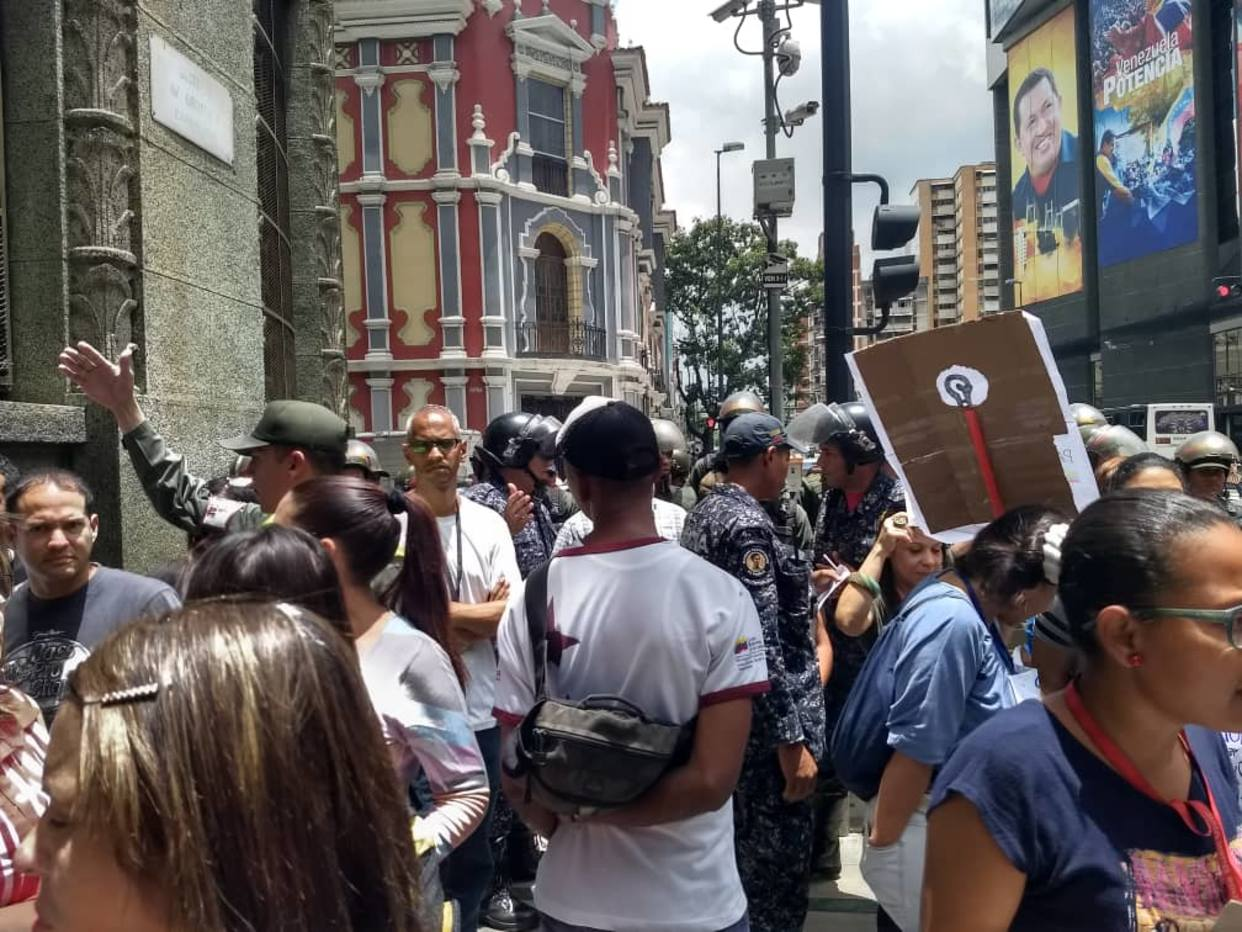
\includegraphics[width=300px]{124.jpg}%
\newline%
%
El sector público fue el blanco del chavismo para aplicar su modelo laboral corporativo, que emprendió en 2007 con la implantación de un contrato colectivo único en las instituciones del Estado, el cual incluía la reducción de los niveles y grados en las escalas y tabuladores y otros beneficios laborales, aseguraron fuentes sindicales.%
\newline%
%
“Las desmejoras en el pago de los salarios, las primas y las compensaciones se hicieron cada vez más frecuentes y los trabajadores salían a protestar por sus derechos. Sin embargo, la última tabla salarial vigente a partir del 1º de este mes es el colmo del abuso”, afirmó Pablo Zambrano, coordinador del Movimiento de Sindicatos de Base.%
\newline%
%
La implantación unilateral y arbitraria del gobierno de la nueva escala salarial se convirtió en punto de honor para la protesta nacional de trabajadores, convocada para hoy por las organizaciones sindicales y gremiales no oficialistas y que incluye varias acciones de calle. Los maestros harán pancartazos en las puertas de los planteles públicos, mientras que el gremio de profesores de educación superior convocó a una concentración en~la Plaza~del Rectorado de~la Universidad~Central de Venezuela.%
\newline%
%
Los trabajadores de~la salud~protestarán frente a los centros hospitalarios y los de~la Corporación~Eléctrica~Nacional y de~la Cantv~se congregarán al final de~la avenida~Libertador en Caracas. También se prevé una concentración frente a la sede de~la Confederación~de Trabajadores de Venezuela.%
\newline%
%
El representante de Mosbase destacó que las acciones de hoy serán para demostrar cómo el presidente Nicolás Maduro trató de engañar a los trabajadores con el alza del salario mínimo de 3 millones a 180 millones de bolívares anteriores, esto es, de~30 a~1.800 bolívares soberanos a partir del 1° de este mes.%
\newline%
%
“El gobierno se agarró de ese aumento para implantar un nuevo tabulador mediante un instructivo, aún no publicado en~Gaceta Oficial, que reduce las diferencias de sueldos entre los tramos de las escalas y desmejora y hasta elimina primas y otros beneficios conquistados por los trabajadores en sus luchas”, dijo Zambrano.%
\newline%
%
Pablo Alzuru, presidente de~la Federación~Venezolana~de Maestros, precisó que el tabulador anterior de los docentes se iniciaba con más de 8 salarios mínimo, pero ahora es uno solo de 1.800 bolívares mensuales. Agregó que como al resto de los organismos del Estado, el gobierno les impuso la tabla del instructivo que elaboró para la administración pública.%
\newline%
%
Víctor Márquez, de~la Asociación~de Profesores de~la Universidad~Central~de Venezuela, indicó que el tabulador previo abría con 4,5 salarios mínimo, pero en los 2 pagos iniciales de septiembre el arranque fue 1.800 bolívares, además de las rebajas u omisiones de primas y beneficios.%
\newline%
%
Con el instructivo, el gobierno irrespetó los contratos colectivos sectoriales como los del sector eléctrico y las empresas básicas de Guayana, cuyo comienzo es de 1,5 salarios mínimo y de 16,5\% a 25\% adicional al sueldo mínimo.%
\newline%
%
Zambrano señaló que en la tabla del sector público la diferencia anterior entre los niveles de 6\% fue bajada a 2\%. “Las prima de antigüedad (entre 10\% y 60\%) fue llevada a 1\% y 30\% del sueldo mínimo. Eliminaron la de transporte, becas y útiles escolares”.%
\newline%
%
Servando Carbone, dirigente de~la Unión Nacional~de Trabajadores, denunció que en una reunión del 31 de agosto el Ejecutivo entregó a todos los directores de Recursos Humanos de los órganos estatales el instructivo con las escalas de salarios para “aplicarlas sin rechistar”.%
\newline%
%
Las fuentes sindicales consultadas criticaron “las posiciones antiobreras y defensa del gobierno” de dirigentes laborales, pero que pertenecieron antes a partidos opositores.%
\newline%
%
Wills Rangel, presidente de~la Central~Bolivariana~Socialista de Trabajadores y de~la Federación~Nacional~de Trabajadores Petroleros de Venezuela, declaró el 10 de septiembre:~“Es hora de que en el país se haga una sola tabla o un solo régimen salarial de acuerdo con las cualidades y conocimientos de cada persona”.%
\newline%
%
Quién es quién%
\newline%
%
Wills Rangel%
\newline%
%
Presidente de~la Central Bolivariana~Socialista de Trabajadores y de~la Futpv. Viene~de Acción Democrática y fue mano derecha de Carlos Ortega, ex presidente de~la Fedepetrol. Está~en la milicia obrera y es constituyente.%
\newline%
%
Franklin Rondón%
\newline%
%
Constituyente. Militó en Copei y fue dirigente de~la Federación~de Empleados Públicos, afiliada a~la CTV. Chavista~desde 2002, en 2004 fundó~la Federación Nacional~de Trabajadores del Sector Público.%
\newline%
%
Francisco Torrealba%
\newline%
%
Estuvo en Acción Democrática. Presidió el Sindicato del Metro de Caracas y fue diputado del PSUV en 2016. Es constituyente. Fue ministro del Trabajo entre enero y mediados de 2017.%
\newline%
%
\end{document}